\documentclass{beamer}


\usepackage{amsmath}
\usepackage[style=alphabetic,url=true]{biblatex}
\usepackage{environ}
\usepackage{geometry}
\usepackage{graphicx}
\usepackage{tikz}
\usepackage[T2A]{fontenc}
\usepackage[utf8]{inputenc}
\usepackage[cache=false]{minted}
\usepackage{amsmath}
\usepackage{amsfonts}
\usepackage{amssymb}
\usepackage{calrsfs}
\usepackage{animate}
\usepackage{xmpmulti}


% \usetheme{Bergen}

\usecolortheme{beaver}

\setbeamertemplate{itemize item}[circle]
\setbeamertemplate{itemize subitem}{--}
\addtobeamertemplate{navigation symbols}{}{
  \usebeamerfont{footline}%
  \usebeamercolor[fg]{footline}%
  \hspace{1em}%
  \insertframenumber/\inserttotalframenumber
}
\graphicspath{ {./graphics/} }
\setminted[Python]{
  fontsize=\tiny
}
\BeforeBeginEnvironment{minted}{\medskip}
\AfterEndEnvironment{minted}{\medskip}
\usetikzlibrary{matrix}
\tikzset{
  stack/.style={
    matrix of nodes,
    nodes={
      fill=lightgray,draw,text=black,font=\sffamily\bfseries,
      text height=11pt,text depth=3pt,baseline=center, minimum width=1cm
    },
    column sep=-\pgflinewidth/2
  }
}

\title{
  Біткоїн та криптовалютні технології \\
  Лекція 6: Біткоїн-мережа
}

\author{Юрій Жикін}
\date{17 березня, 2025}

\begin{document}

\frame{\titlepage}

\begin{frame}
  \frametitle{Однорангові мережі 1/2}
  \begin{itemize}
  \item \textbf{Однорангова} \textbf{мережа} (\textbf{P2P-мережа}) - це система,
    яка розподіляє завдання або навантаження між \textit{рівноправними},
    \textit{рівноцінними} вузлами, що називаються \textit{пірами} або просто
    \textit{вузлами}.
  \end{itemize}
  \begin{center}
    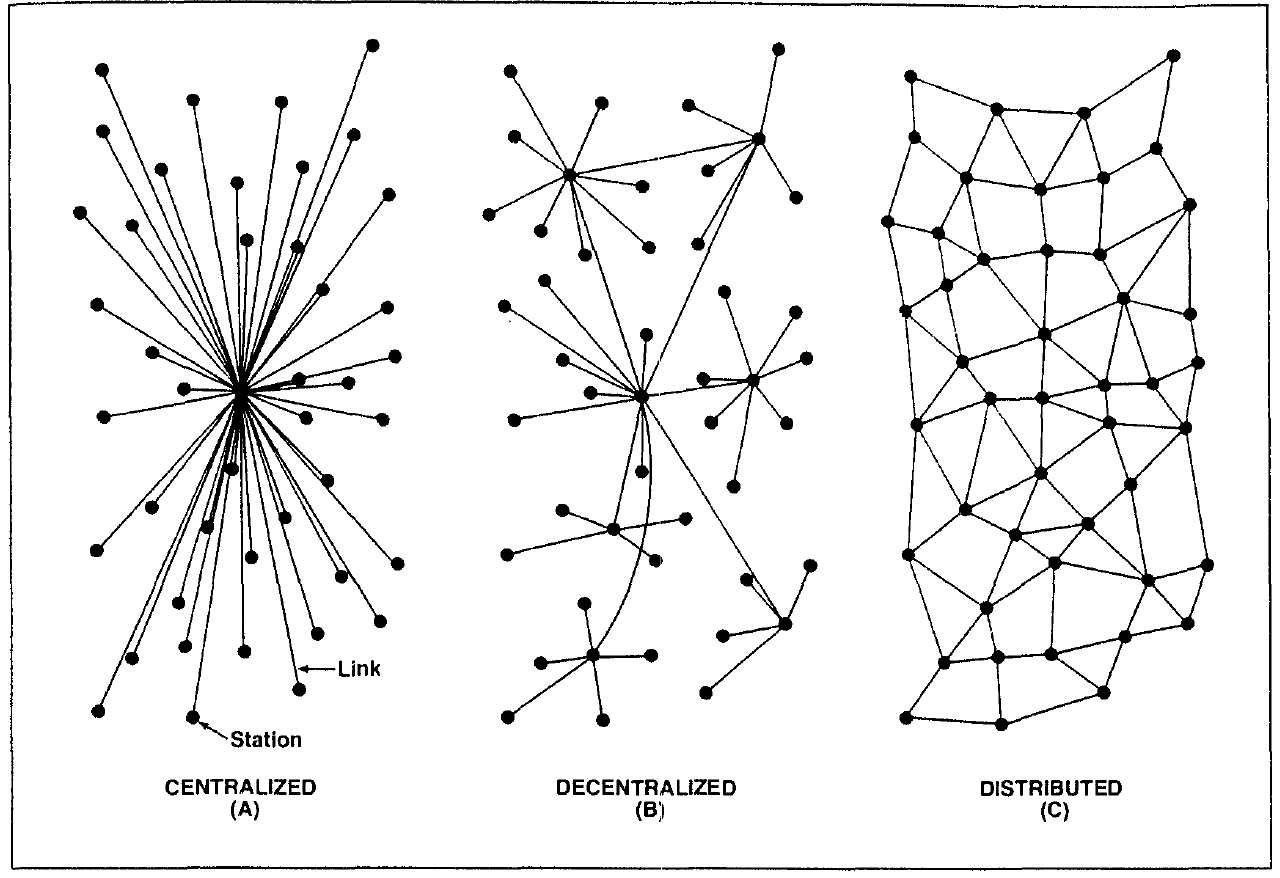
\includegraphics[width=0.8\textwidth]{networks}
  \end{center}
\end{frame}

\begin{frame}
  \frametitle{Однорангові мережі 2/2}
  \begin{itemize}
  \item У \textbf{централізованих} системах успішна атака на \textbf{сервер}
    виводить з ладу всю систему.
  \item У \textbf{децентралізованих} системах успішна атака на \textbf{вузол}
    призводить до тимчасового поділу мережі, але система продовжує
    функціонувати.
  \item У \textbf{однорангових} системах успішна атака на \textbf{вузол} не
    впливає на мережу, \textit{якщо мережа достатньо велика}.
  \item Приклади: \textbf{Napster} та \textbf{BitTorrent}.
  \end{itemize}
\end{frame}

\begin{frame}
  \frametitle{Біткоїн-мережа 1/2}
  \begin{itemize}
  \item \textbf{Біткоїн-мережа} - це \textbf{однорангова} мережа, що складається
    з \textbf{Біткоїн-вузлів}, які поширюють блоки та транзакції за допомогою
    \textbf{протоколу пліток} і перевіряють їх відповідно до \textbf{правил
      консенсусу}.
  \item Згідно з \href{https://bitnodes.io}{bitnodes.io}, Біткоїн-мережа має
    приблизно \textbf{21,000} \textit{досяжних} вузлів, порівняно з 16,000 у
    2022 році та 10,000 у 2021 році.
  \item Згідно з \href{https://luke.dashjr.org}{luke.dashjr.org}, загальна
    кількість \textbf{повних} вузлів (тобто вузлів, що здійснюють перевірку
    даних ланцюга блоків) оцінюється приблизно у \textbf{100,000} вузлів.
  \end{itemize}
\end{frame}

\begin{frame}
  \frametitle{Біткоїн-мережа 2/2}
  \begin{itemize}
  \item Згідно з \href{https://luke.dashjr.org}{luke.dashjr.org}, 71.62\% усіх
    вузлів працюють на найновішому програмному забезпеченні (Bitcoin Core 28.x,
    27.x).
  \end{itemize}
  \begin{center}
    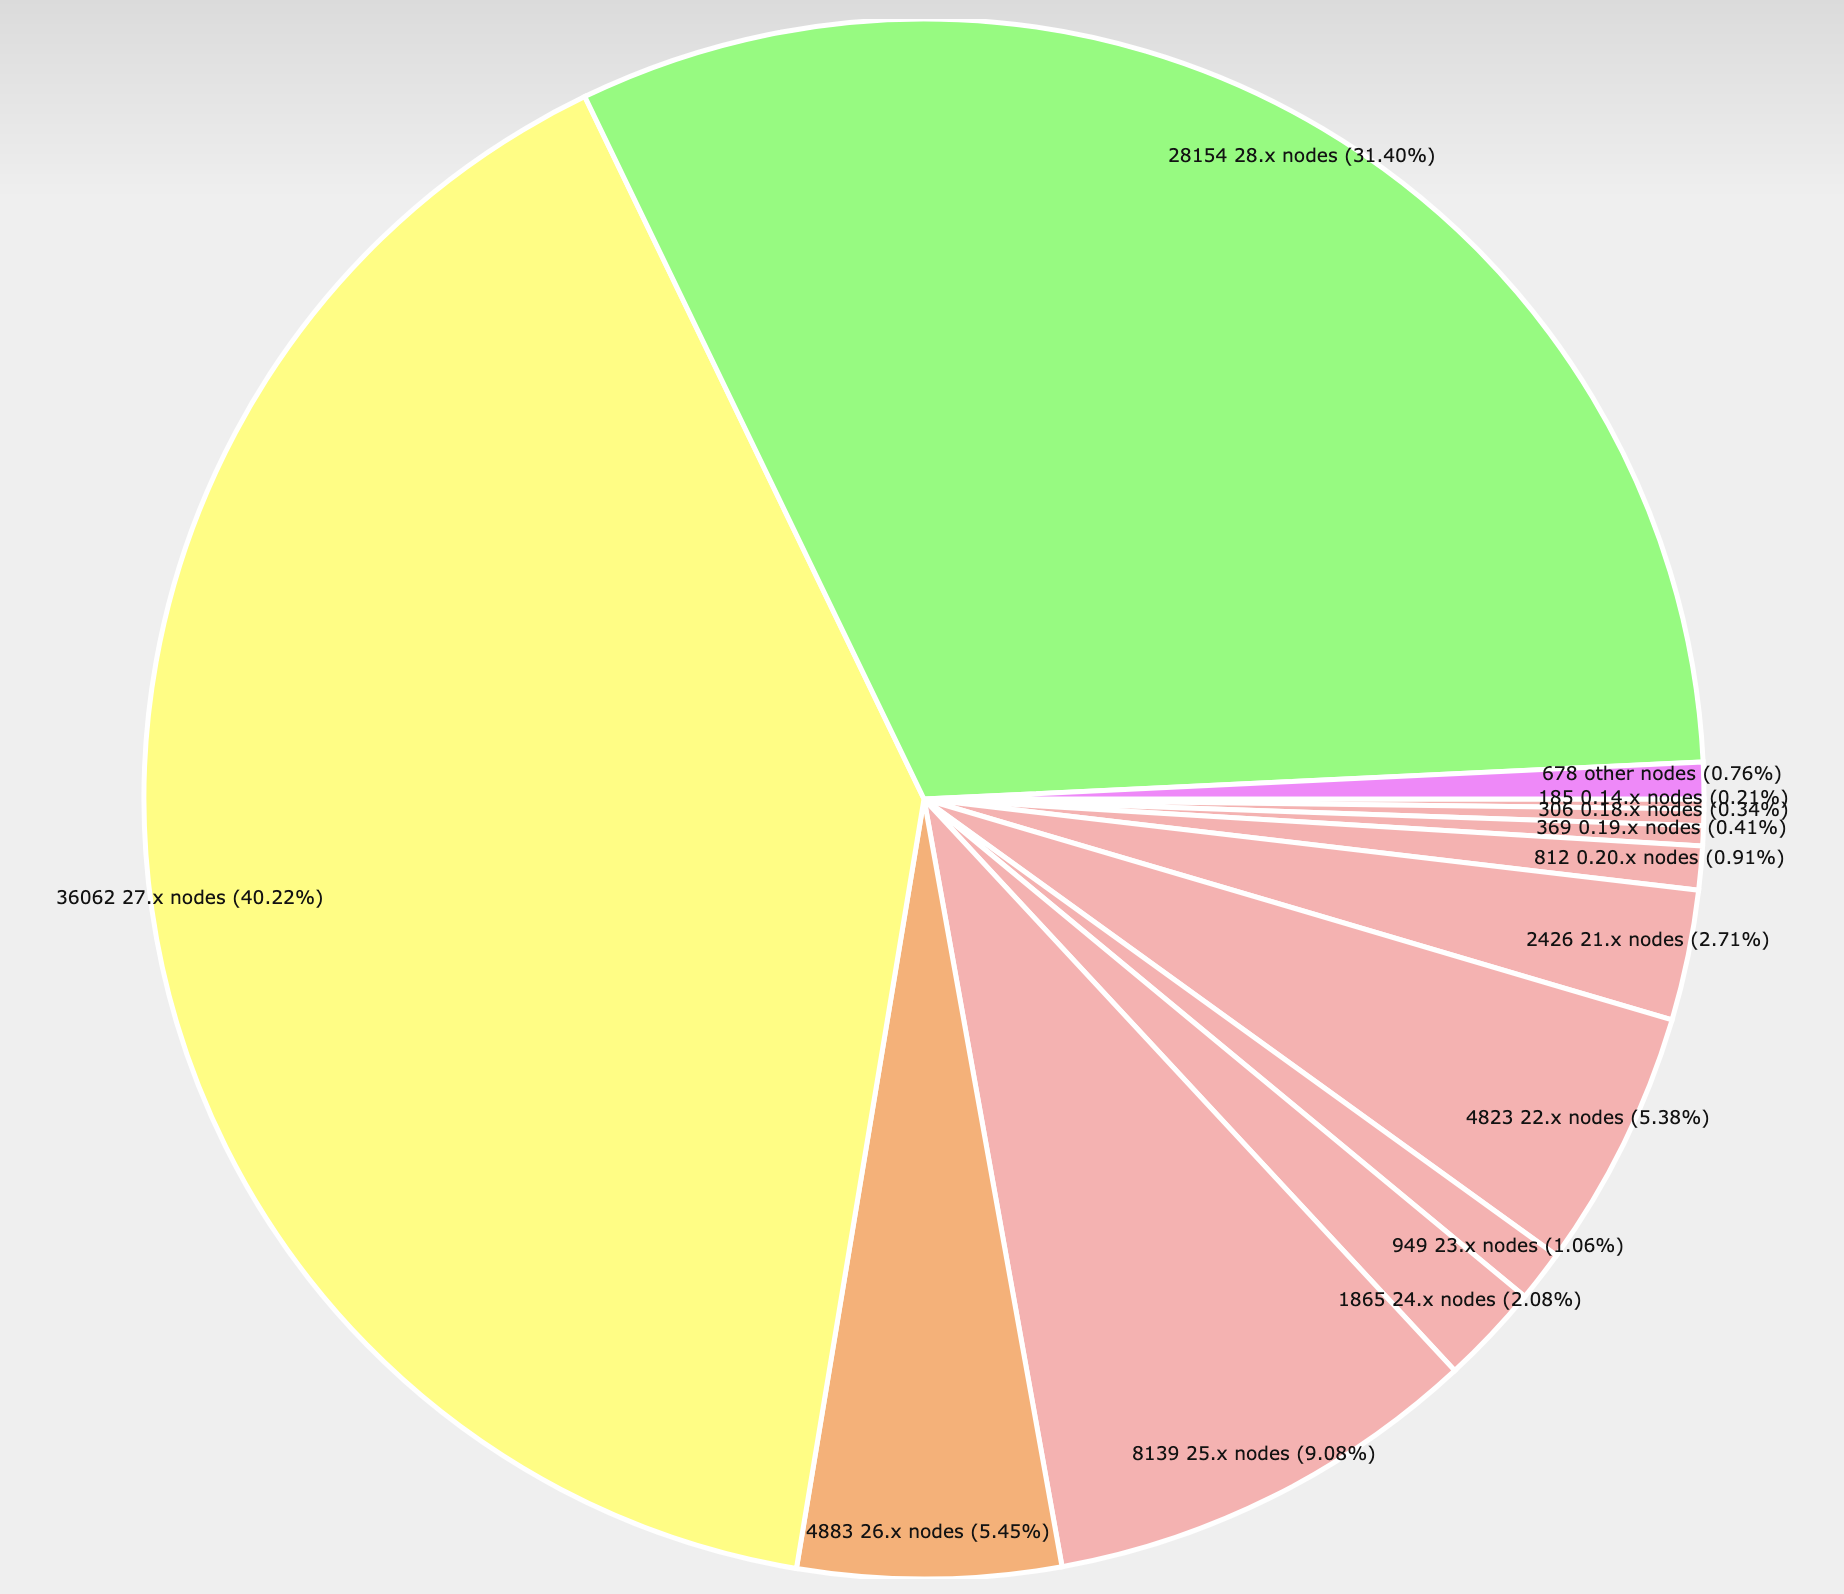
\includegraphics[width=0.7\textwidth]{nodes}
  \end{center}
\end{frame}

\begin{frame}
  \frametitle{Протокол пліток}
  \begin{itemize}
  \item \textbf{Протокол пліток} (\textbf{епідемічний протокол}) - це процес
    однорангової комунікації, заснований на принципі поширення пліток (або
    епідемій).
  \item \textbf{Отримання інформації від одного з сусідів і передача її
      якомога більшій кількості інших сусідів.}
  \item \textbf{Протокол пліток Біткоїн-системи} - це протокол поширення нових
    блоків і транзакцій у Біткоїн-мережі, який також забезпечує надання старих
    блоків з сховища новим вузлам.
  \end{itemize}
  \begin{center}
    \transduration<0-6>{0}
    \multiinclude[<+->][format=png, graphics={width=0.5\textwidth}]{gossip}
  \end{center}
\end{frame}

\begin{frame}
  \frametitle{Вузол Біткоїн-мережі}
  \begin{itemize}
  \item \textbf{Біткоїн-вузол} - це учасник мережі Bitcoin, програмне
    забезпечення, яке перевіряє блоки та транзакції і ``пліткує'' з іншими
    учасниками.
  \item Новий Біткоїн-вузол:
    \begin{itemize}
    \item ініціалізує з'єднання з кількома вузлами через DNS-сервери,
    \item виконує \textbf{початкове завантаження блоків} (\textbf{IBD}),
    \item створює необхідні індекси (множина UTXO),
    \item починає прослуховування пліток про нові блоки і транзакцій,
    \item відхиляє недійсні блоки та транзакції,
    \item приймає та ретранслює дійсні блоки і транзакції.
    \end{itemize}
  \end{itemize}
\end{frame}

\begin{frame}
  \frametitle{Реорганізація ланцюга 1/2}
  \begin{itemize}
  \item Коли вузол отримує новий блок, який не належить до поточного ланцюга,
    він намагається під'єднати його до ланцюга, знайшовши \textbf{точку
      розгалуження}.
  \item Після під'єднання блоку, \textbf{ланцюг, на створення якого було
      витрачено більше енергії} (ланцюг з найбільшою \textbf{сукупною роботою}),
    обирається як дійсний ланцюг.
  \end{itemize}
  \begin{center}
    \begin{tikzpicture}
      % Define block size
      \def\blocksize{0.6}

      % Define colors
      \definecolor{mainchain}{RGB}{0,0,0}
      \definecolor{forkchain}{RGB}{200, 200, 200}
      \definecolor{genesis}{RGB}{50,100,100}

      % Genesis block
      \node[draw, fill=genesis, minimum size=\blocksize cm] (G) at (-1,0) {};

      % Main chain blocks
      \node[draw, fill=mainchain, minimum size=\blocksize cm] (B1) at (0,0) {};
      \node[draw, fill=mainchain, minimum size=\blocksize cm] (B2) at (1,0) {};
      \node[draw, fill=mainchain, minimum size=\blocksize cm] (B3) at (2,0) {};
      \node[draw, fill=mainchain, minimum size=\blocksize cm] (B4) at (3,0) {};
      \node[draw, fill=mainchain, minimum size=\blocksize cm] (B5) at (4,0) {};
      \node[draw, fill=mainchain, minimum size=\blocksize cm] (B6) at (5,0) {};
      \node[draw, fill=mainchain, minimum size=\blocksize cm] (B7) at (6,0) {};
      \node[draw, fill=mainchain, minimum size=\blocksize cm] (B8) at (7,0) {};

      % Forks
      \node[draw, fill=forkchain, minimum size=\blocksize cm] (F1) at (1, 1) {};
      \node[draw, fill=forkchain, minimum size=\blocksize cm] (F2) at (4,-1) {};
      \node[draw, fill=forkchain, minimum size=\blocksize cm] (F3) at (5,-1) {};
      \node[draw, fill=forkchain, minimum size=\blocksize cm] (F4) at (6, 1) {};

      % Connecting lines
      \draw[-] (G) -- (B1);
      \draw[-] (B1) -- (B2);
      \draw[-] (B2) -- (B3);
      \draw[-] (B3) -- (B4);
      \draw[-] (B4) -- (B5);
      \draw[-] (B5) -- (B6);
      \draw[-] (B6) -- (B7);
      \draw[-] (B7) -- (B8);

      % Fork connections
      \draw[-] (B1) -- (F1);
      \draw[-] (B4) -- (F2);
      \draw[-] (F2) -- (F3);
      \draw[-] (B6) -- (F4);

      % Labels
      \node[above] at (-1,0.3) {Генезис};
      \node[above] at (1, 1.3) {Відгалуження 1};
      \node[below] at (5,-1.3) {Відгалуження 2};
      \node[above] at (6, 1.3) {Відгалуження 3};

    \end{tikzpicture}
  \end{center}
\end{frame}

\begin{frame}
  \frametitle{Реорганізація ланцюга 2/2}
  \begin{itemize}
  \item \textbf{Робота ланцюга} (англ. \textbf{сhainwork}) - це загальна
    кількість операцій хешування, яку було необхідно здійснити для створення
    поточного ланцюга (за оцінкою).
  \item \textbf{Початкове завантаження заголовків блоків}
    (англ. \textbf{headers-first IBD mode}) робить початкове завантаження блоків
    (IBD) ефективнішим, завантажуючи спочатку весь ланцюг у вигляді заголовків,
    а вже потім завантажуючи повні блоки для сконструйованого ланцюга.
  \end{itemize}
\end{frame}

\begin{frame}
  \frametitle{Мемпул}
  \begin{itemize}
  \item \textbf{Мемпул} (англ. \textbf{mempool}) - це структура даних у пам'яті,
    яка містить усі відомі дійсні транзакції, що ще не були включені до жодного
    блоку.
  \item Вузли підтримують \textbf{комбінована множина UTXO}, який складається з
    усіх UTXO у ланцюзі та всіх UTXO у мемпулі.
  \item Коли вузол отримує нову дійсну транзакцію, він додає її до мемпула.
  \item Коли вузол отримує новий дійсний блок, він видаляє з мемпула усі
    транзакції, що містяться в цьому блоці.
  \item Коли вузол отримує нову транзакцію, яка конфліктує з транзакцією у
    мемпулі, він відхиляє нову транзакцію, якщо вона не відповідає правилам
    \textbf{заміни за комісією} (англ. \textbf{RBF} - \textbf{Replace By Fee}).
  \end{itemize}
\end{frame}

\begin{frame}
  \frametitle{Майнінг}
  \begin{itemize}
  \item \textbf{Майнінгові вузли} - це звичайні вузли, які створюють нові блоки
    з транзакцій у mempool.
  \item Майнер вибирає певну кількість транзакцій (2000-4000, зазвичай у порядку
    зменшення комісії) для створення \textbf{шаблону блоку} відповідно до
    \textbf{обмеження розміру}.
  \item Майнінгове обладнання виконує обчислення методом грубої сили
    \textbf{доказу виконаної роботи} (\textbf{Proof of Work}) :
    $HASH256(Block) < Target$.
  \item Коли (якщо) блок ``добуто'' (тобто знайдено рішення PoW), майнер
    надсилає його в мережу через протокол пліток.
  \item Якщо інший майнер одночасно ``добуває'' інший блок, мережа вирішує
    конфлікт через реорганізацію ланцюга.
  \end{itemize}
\end{frame}

\begin{frame}
  \frametitle{Життєвий цикл транзакції 1/2}
  \begin{itemize}
  \item Транзакція \textbf{знищує} певну частину UTXO у ланцюзі та мемпулі і
    \textbf{створює} нову множину UTXO у мемпулі.
  \item \textbf{Фіналізована} дійсна транзакція поширюється через протокол
    пліток по всій мережі.
  \item Транзакція зазвичай залишається в мемпулі, доки її комісія не перевищить
    поріг включення у наступний блок.
  \item Поки транзакція знаходиться в мемпулі, її можна ``підняти'' в черзі за
    допомогою:
    \begin{itemize}
    \item \textbf{заміни за комісією} (\textbf{Replace By Fee}, \textbf{RBF}), або
    \item \textbf{``нащадок платить за предка''} (\textbf{Child Pays For
        Parent}, \textbf{CPFP}).
    \end{itemize}
  \end{itemize}
\end{frame}

\begin{frame}
  \frametitle{Життєвий цикл транзакції 2/2}
  \begin{itemize}
  \item Рано чи пізно транзакція потрапляє в один із блоків.
  \item Після того як цей блок ``здобуто'' та поширено мережею, кожен вузол у
    мережі:
    \begin{itemize}
    \item видаляє транзакцію з свого мемпулу,
    \item застосовує транзакцію до множини UTXO (видаляє знищені UTXO та
      додає створені).
    \end{itemize}
  \item На цьому етапі транзакція вважається \textbf{підтвердженою}.
  \end{itemize}
\end{frame}

\begin{frame}
  \frametitle{Кінець}
  \begin{center}
    Дякую за увагу!
  \end{center}
\end{frame}

\end{document}

%%% Local Variables:
%%% mode: latex
%%% TeX-master: t
%%% End:
